\section{QNodeOS Design and Implementation}
\label{qnodeos:sec:design}

We proceed with a more detailed description of the \ac{QNodeOS} architecture and implementation, where (for the reader's convenience) we include some information already found in \cref{qnodeos:sec:architecture,qnodeos:sec:methods}. Recall, that a quantum network application is realized by running separate programs, one on each end node of the quantum network that takes part in the quantum application. The individual programs interact with each other only via classical message passing and entanglement generation. Each program itself consists of classical and quantum blocks of code (see~\cref{qnodeos:sec:design-consid:challenges:application}) which require execution in the quantum memory for the application to succeed.

\subsection{QNodeOS Architecture}
\label{qnodeos:sec:appendix-arch}

\subsubsection{Quantum Network Node System}
\label{qnodeos:sec:appendix-arch-node_system}

We remark that \ac{QNodeOS}---a real-time system for quantum network nodes---is designed to be deployed on end and intermediary nodes (\cref{qnodeos:sec:quantum-networks}), where \ac{QNodeOS} use on intermediary nodes can be restricted to facilitate entanglement generation over the network via a (series) of intermediate nodes.
As the focus of this work is the execution of quantum network application, we focus here on running \ac{QNodeOS} on end nodes.

In our model, as depicted in~\cref{qnodeos:fig:fig2}a, we divide the functions of a node into three high-level components:

\begin{itemize}
\item a \emph{\ac{CNPU}}, on which classical blocks of code are executed. The \emph{CNPU} is required at end nodes, and requires classical computing hardware (including a classical \ac{CPU}), as well as a classical network device to allow the exchange of messages with the \ac{CNPU} of remote nodes. While quantum networking programs can in principle be developed and compiled outside of the \ac{CNPU}), the \emph{CNPU} may also realize a user environment where quantum networking programs (refer to \cref{qnodeos:sec:design:network-application}) are developed and compiled, and where program results are stored; 
\item a \emph{\ac{QNPU}}, which receives quantum blocks from the \ac{CNPU} and entanglement generation requests from peer nodes, and manages execution on the quantum physical device; 
\item a \emph{\ac{QDevice}}---the quantum physical device---consisting of a quantum processor, a quantum network device, and a quantum memory, where actual quantum computations and communications take place. In present-day quantum hardware implementations, the same device acts as a quantum processor, a network device and a memory.
\end{itemize}

In summary, in our design a quantum network program starts on the general-purpose \ac{OS}, i.e. a \ac{CNPU}, which runs classical code blocks internally, and offloads quantum code blocks to the \ac{QNPU}. The \ac{QNPU} runs the quantum code blocks, relying on the underlying quantum device, i.e., \ac{QDevice}, to execute the actual quantum operations. 

\ac{CNPU} and \ac{QNPU}---while both being capable of performing non-quantum operations---are conceptually separate components, with the main difference being that the \ac{QNPU} is expected to meet real-time requirements (to enable entanglement generation) and perform its arbitration tasks within set deadlines, whereas the \ac{CNPU} does not need to provide such guarantees. This is because the QNPU should adhere to a network schedule which imposes real-time requirements. \ac{CNPU}, \ac{QNPU} and \ac{QDevice} have a classical connection to their counterpart at the remote node, where the \ac{QDevice} also has an additional optical fiber connection to the quantum network to perform quantum operations.

An implementation of the quantum network node could have these three top-level components (\ac{CNPU}, \ac{QNPU} and \ac{QDevice}) deployed on three physically distinct environments, or group some of them on the same chip or board. Furthermore, classical and quantum code blocks can be run on a single system, provided that this system has a connection to the quantum device to execute the actual quantum instructions. However, in the interest of a simpler implementation, where each system has a scoped responsibility, we opted to map classical and quantum blocks onto two distinct environments. Classical blocks are run on a system that features a fully-fledged \ac{OS} (here, Linux), with access to high level programming languages (like C++ and Python) and libraries. Quantum blocks are delegated to the \emph{\ac{QNPU}}, which is a system capable of interpreting quantum code blocks and managing the resources of a quantum device. 

We note that the \ac{QNPU} itself is an entirely classical system that interacts with the quantum hardware (the \ac{QDevice}). At the moment, our implementation of the \ac{QNPU} is fully software, including the instruction processor. In general, the system may be implemented entirely in software running on a classical \ac{CPU}, or parts of its functionality may be implemented in classical hardware, e.g.~\ac{FPGA} (see the description of the trapped-ion platform implementation in~\cref{qnodeos:sec:trapped-ion-platform}) or \ac{ASIC}.

\subsubsection{Quantum Network Programs}
\label{qnodeos:sec:design:network-application}

A quantum networking user program is what a programmer writes on the \ac{CNPU}, in a high-level language, through the use of some \ac{SDK}. Classical code blocks can in principle be programmed in any language yielding an executable suitable to run on the \ac{CNPU}. Fully-classical code blocks---which include local processing and communication with other end nodes---often produce input data for the next quantum code blocks. That is, a classical code block typically precedes a quantum code block whose instructions depend on external data coming from a remote end node. In the future, quantum blocks could include real-time execution constraints, for example, a deadline by which execution should be completed in order to reach a specific application performance while the quantum memory has a limited memory lifetime.

\paragraph{NetQASM} To express quantum code blocks, we make use of \emph{\ac{NetQASM}}~\cite{dahlberg_2022_netqasm} as an instruction set for quantum network programs, which is described in detail in~\cite{dahlberg_2022_netqasm}. 
Before this work, \ac{NetQASM} has only ever been used to execute quantum network programs on simulated quantum network nodes, and has never been realized on hardware to execute quantum network applications.

The instruction set used in \ac{NetQASM} for the quantum code blocks is similar to other \ac{QASM} languages (see e.g. Refs.~\cite{cross_2017_qasm,khammassi_2018_cqasm,fu_2019_eqasm}), but it is extended to include instructions for quantum networking. We emphasize that \ac{NetQASM} is not a strict requirement of \ac{QNodeOS}, and other ways to express quantum code blocks could be used in other implementations. The instruction set of this language should support both computational and networking quantum instructions, as well as simple classical arithmetic and branching instructions to be used for real-time processing on the \ac{QNPU}. It is the compiler's task to transform high-level blocks for the \ac{QNPU} into \ac{NetQASM} blocks. 

\ac{NetQASM} defines a notion of \ac{NetQASM} subroutines, where each subroutine corresponds to a quantum block of code, specified by the compiler or programmer. We therefore use the term \emph{quantum block} to refer to a \emph{NetQASM subroutine} in the remainder of this text. A full list of operands that can appear in a \ac{NetQASM} subroutine is given in~\cite[Appendix B]{dahlberg_2022_netqasm}. \ac{NetQASM} assumed subroutines would be executed on a form of \ac{QNPU} (without specifying an architecture for the \ac{QNPU}), potentially using a form of shared memory with \ac{CNPU}. In the absence of a shared memory, \ac{NetQASM} allowed classical variables inside subroutines to be kept on the \ac{QNPU}, and accessed read-only by the \ac{CNPU} via the \ac{NetQASM} interface (see below). The \ac{CNPU} can also specify classical constants for the use inside subroutines, as part of submitting a subroutine to the \ac{QNPU}.

We use here the \ac{NetQASM} \ac{SDK}~\cite{netqasm_sdk} to write programs, where the \ac{SDK} compiles a quantum network program, written in Python, into a series of classical and quantum code blocks. This \ac{SDK} was previously used to express programs on a simulated quantum network~\cite{squidASM}.

\paragraph{NetQASM Interface}

Our interface between the \ac{CNPU} and the \ac{QNPU} (\cref{qnodeos:sec:QNPU-api}) includes the \ac{NetQASM} interface defined in~\cite[Appendix A]{dahlberg_2022_netqasm}.
This interface in particular allows the \ac{CNPU} to register a program on the \ac{QNPU}, submit \ac{NetQASM} subroutines, and access the results of said subroutines.

\subsubsection{Program Processing Pipeline}

\paragraph{CNPU Processing}

When a program start execution on the \ac{CNPU}, a new \ac{CNPU} process is created. As we separate the \ac{CNPU} from the \ac{QNPU} in our implementation, it is natural to rely on the properties of an existing classical operating system to take care of this function. In our implementation, we start a single program on the \ac{CNPU} which then creates a thread (using standard Linux thread library~\cite{linux_threads} for each \ac{CNPU} process. The classical blocks belonging to the \ac{CNPU} program are executed locally on the \ac{CNPU}. These may involve some form of coordination with the remote \ac{CNPU} of the user program, as well as pre- or post-processing of the results coming from \ac{NetQASM} subroutines. While this can also be done later, when the program starts it will typically also establish a TCP/IP connection with the program running on the remote \ac{CNPU} leading to the establishment of a TCP/IP socket that will be used for classical application level communication between the \acp{CNPU}.

The \ac{CNPU} then registers the program on the \ac{QNPU}. Later, \ac{NetQASM} subroutines of these programs are sent from the \ac{CNPU} to the \ac{QNPU} through the \emph{\ac{NetQASM} interface}. 

\paragraph{QNPU Processing}

When a program is registered with the \ac{QNPU} by the \ac{CNPU}, the \ac{QNPU} creates a user process to store program data and execution state. The \ac{QNPU} also keeps track of \ac{NetQASM} subroutines belonging to the user process, which may be submitted only later, as well as other run-time data analogous to what a typical process control block contains, useful for the execution of the program. As depicted in~\cref{qnodeos:fig:fig2}a, a subroutine can, in general, be composed of three classes of instructions:

\begin{itemize}
\item \emph{Quantum operations}: quantum physical operations, to be performed on the underlying quantum device;
\item \emph{Classical logic}: arithmetic and branch instructions, to be executed in-between quantum operations, useful to store results of quantum operations and to perform responsive decision-making;
\item \emph{Entanglement requests}: requests to generate an entangled qubit pair with a remote node in the network.
\end{itemize}
%
Classical logic is processed locally on the \ac{QNPU}, and potentially results in the update of a process's data. This data includes \ac{NetQASM} variables capturing measurement results, for example, that may latter be conveyed to the \ac{CNPU}. 

When the user process starts on the \ac{QNPU} an \ac{ER} socket (see~\cref{qnodeos:sec:design_er_socket}) is established with the remote \ac{QNPU} that is used to associate later entanglement requests with the specific user process. Entanglement requests contained in the \ac{NetQASM} subroutines are forwarded to the quantum network stack,  which stores them together with other requests coming from network peers. Entanglement generation requests coming from other nodes in the network are received on the quantum network stack through the \emph{\ac{QNetStack} interface}.

Quantum instructions are sent to the \ac{QDevice} through the \ac{QDriver}, which provides an abstraction of the \ac{QDevice} interface. The \ac{QDriver} translates \ac{NetQASM} instructions into physical instructions suitable to the underlying physical platform.

\paragraph{QDevice Processing}

Physical instructions are executed on the \ac{QDevice}, the quantum processing and networking unit. The \ac{QDevice} processing stack heavily depends on the underlying physical platform---for instance, \ac{NV} centers in diamond, or Trapped Ions.

As we remarked in~\cref{qnodeos:sec:appendix-arch-node_system}, a \ac{QDevice} has two communication channels with its direct neighbors: a \emph{classical channel}, used for low-level synchronization of the entanglement generation procedure and other configuration routines, and a \emph{quantum channel}, typically an optical fiber, through which qubits can travel.

\subsection{QNPU Stack}
\label{qnodeos:sec:design:qnpu_stack}

\begin{figure}
\begin{center}
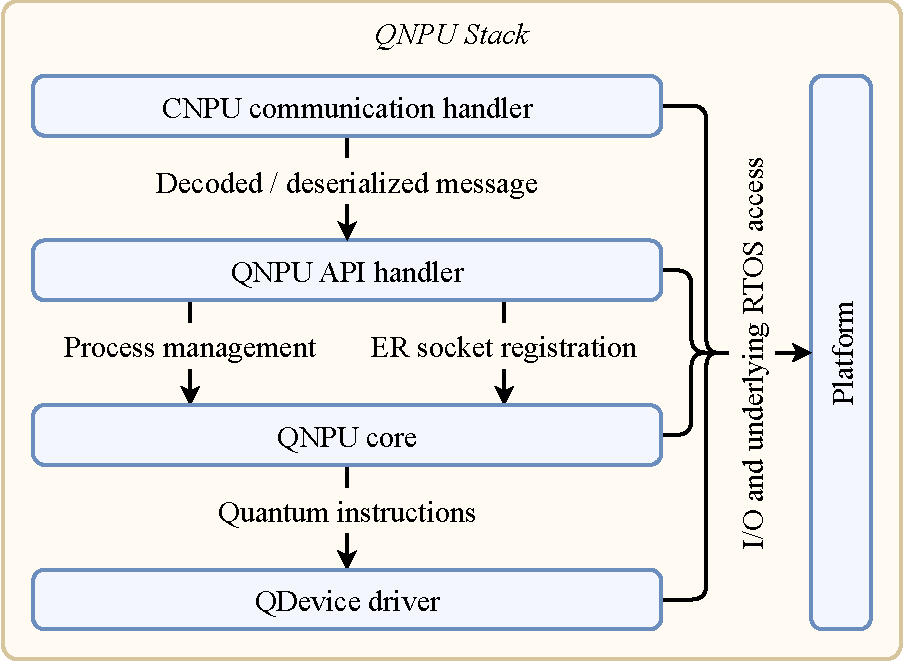
\includegraphics[width=0.6\textwidth]{figures/qnodeos/supplementary/qnodeos-stack.pdf}
\end{center}
\caption[]{\ac{QNPU} stack. The \emph{\ac{QNPU} \acs{API} handler} and \emph{the \ac{QNPU} core} form the central processing layers, and are independent of the underlying quantum physical platform and of the device where \ac{QNodeOS} runs. The \emph{\ac{CNPU} communication handler} translates protocol-specific messages from the \ac{CNPU} into \acs{API} calls. The \emph{\ac{QDevice} driver} (or \ac{QDriver}) abstracts the \ac{QDevice} hardware. The \emph{Platform} layer abstracts the hardware where \ac{QNodeOS} runs, and is accessible to all other layers. Note that three other \ac{API} types are implemented, i.e. \emph{control}, \emph{management}, and \emph{operations}. Control \ac{API} is used for the network schedule, while management and operations \ac{API} are for operational purposes. }
\label{qnodeos:fig:qnodeos-stack}
\end{figure}

\ac{QNodeOS} is a system consisting of multiple abstraction layers, as depicted in \cref{qnodeos:fig:qnodeos-stack}. It is designed to be platform-independent, i.e., independent of the underlying quantum physical platform (quantum hardware) controlled by \ac{QNodeOS}, where connections to different realizations of \ac{QDevice} are captured by a platform-dependent \ac{QDriver}. The implementation of \ac{QNodeOS} itself is of course dependent on the classical physical platform(s) on which \ac{QNodeOS} is implemented, including the physical interface between the \ac{CNPU} and \ac{QNPU}.

\subsubsection{QNPU API}
\label{qnodeos:sec:QNPU-api}

At the center of the stack lie the \emph{the \ac{QNPU} \ac{API} handler} layer and the \emph{the \ac{QNPU} core} layer. The \ac{API} handler is responsible for listening to system calls made to the the \ac{QNPU} \ac{API}, and to relay these calls to the appropriate component inside of the core layer. Such system calls may originate from the \ac{CNPU} via the \emph{CNPU communication handler}, see again~\cref{qnodeos:fig:qnodeos-stack}. 

The \ac{QNPU} \ac{API} is the central engine for managing the execution of local quantum operations and entanglement requests, and manages the hardware resources of the \ac{QDevice}. The \ac{QNPU} \ac{API} exposes services to:
%
\begin{itemize}
\item \emph{Register and deregister a program on the \ac{QNPU}}; This is part of the \ac{NetQASM} interface (see~\cref{qnodeos:sec:design:network-application}).
\item \emph{Add a quantum block (subroutine) for a user process}; This is again part of the \ac{NetQASM} interface.
\item \emph{Open an \ac{ER} socket with a remote node} (\ac{NetQASM} interface).
\item \emph{Control to configure the quantum network stack}, i.e., to configure the network schedule; This is used for the interaction with a network controller that sets network-wide entanglement schedules, as presented in Ref.~\cite{skrzypczyk_2021_arch}.
\item \emph{Perform management and operations functions.}
\end{itemize}
%
The topmost horizontal layer is the \emph{\ac{CNPU} communication handler}, which implements a \emph{protocol wrapper} around \ac{NetQASM}.
We implement this wrapper protocol using EmbeddedRPC~\cite{erpc} for the on-the-wire definition of the messages (including (de-)serialization)). The communication handler translates protocol-specific messages into \ac{API} calls for the \ac{QNPU}. EmbeddedRPC allows to decouple the interface definition and (de-)serialization from the underlying transport layer. We note that only the transport layer is implementation-specific, which depends on the devices where \ac{CNPU} and \ac{QNPU} are implemented and on what the physical interface between them looks like.\footnote{TCP/IP for now, shared memory in the future.}

The \emph{\ac{QDevice} driver} (\ac{QDriver}) layer, at the bottom of the stack, provides an abstraction of the \ac{QDevice} hardware, and its implementation depends on the nature of the \ac{QDevice} itself, and on the physical communication interface between \ac{QNPU} and \ac{QDevice}. Two \ac{QDevice} implementations may differ in a variety of factors, including what quantum physical platform they feature and what digital controller interfaces with the \ac{QNPU}.

Lastly, the vertical \emph{Platform} layer provides \ac{SoC}-specific abstractions for the \ac{QNPU} to access the physical resources of the platform it is implemented on, including I/O peripherals, interrupts controllers and timers. Additionally, if the \ac{QNPU} is implemented on top of a lower-level operating system, this layer gives access to system calls to the underlying \ac{OS}. The Platform layer is vertical to indicate that it can be accessed by all other \ac{QNPU} layers.

Porting the \ac{QNPU} to a different \ac{SoC} (or similar hardware) boils down to implementing a new platform layer. Deploying the \ac{QNPU} on a different \ac{QDevice}, instead, requires both a new \ac{QDriver} and a compiler---on the \ac{CNPU}---that emits quantum instructions supported by the specific \ac{QDevice}.

\subsection{Processes}
\label{qnodeos:sec:design:processes}

A quantum network program starts on the \ac{CNPU}---there, the \ac{CNPU} environment compiles it into classical and quantum code blocks, and creates a new process associated with the program. In the future, an optimized compilation ahead of execution could produce an executable that includes further information (such as execution deadlines depending on the device's memory lifetimes, as mentioned at the beginning of~\cref{qnodeos:sec:design:network-application}). The \ac{CNPU} then registers the program with the \ac{QNPU} (through the \ac{QNPU}'s end node \ac{API}, see \cref{qnodeos:sec:design:qnpu_stack}), which, in turn, creates its own process associated with the registered program. The process on the \ac{CNPU} is a standard \ac{OS} process, which executes the classical code blocks and interacts, (that is: communicating NetQASM subroutines and their results between \ac{CNPU} and \ac{QNPU}), with the counterpart process on the \ac{QNPU}. This interaction can be done by means of a shared memory (and when no shared memory is physically realized: by an exchange of messages~\cite{dahlberg_2022_netqasm}). On the \ac{QNPU}, a process encapsulates the execution of quantum code blocks of a program with associated context information, such as process owner, process number (ID), process state, and process priority.

In the near-term test applications we execute, the execution time of a program is typically dominated by that of quantum blocks, as entanglement generation is a time-consuming operation. Without advanced quantum repeaters~\cite{RepeaterSurvey}, its duration grows exponentially with the distance between the nodes. For this reason, we focus on the scheduling of quantum blocks only, and thus we only discuss \ac{QNPU} processes (also referred to as \emph{user processes}) from this point onward. Again, this does not exclude that in a future iteration of the design \ac{CNPU} and \ac{QNPU} could be merged into one system, and therefore classical and quantum blocks would be scheduled jointly.

\subsubsection{Process Types and Their Interaction}

\paragraph{QNPU user processes}

The \ac{QNPU} allocates a new \emph{user process} to each quantum network program registered by the \ac{CNPU}. A user process is the program's execution context, and consists of \ac{NetQASM} blocks and other context information---the process control block---including process number (ID), process owner, process state, process scheduling priority, program counter, and pointers to process data structures. Process state and priority determine how processes are scheduled on the \ac{QNPU}. A user process becomes active (ready to be scheduled) as soon as the \ac{QNPU} receives a quantum code block from the \ac{CNPU}. Multiple user processes---relative to different \ac{CNPU} programs---can be concurrently active on the \ac{QNPU}, but only one can be running at any time. A running user process executes its quantum code block directly, except for entanglement requests, which are instead submitted to the quantum network stack and executed asynchronously.

\paragraph{QNodeOS network process}

The \ac{QNPU} also defines \emph{kernel processes}, which are similar to user processes, but are created when the system starts (on boot) and have different priority values. Currently, the only existing kernel process is the \emph{network process}. The network process, owned by the \ac{QNetStack}, handles entanglement requests submitted by user processes, coordinates entanglement generation with the rest of the network, and eventually returns entangled qubits to user processes. The activation of the network process is dictated by a network-wide entanglement generation schedule. Such a schedule defines when a particular entanglement generation request can be processed, and therefore it has intersecting entries on adjacent nodes (given that entanglement is a two-party process). The schedule can be computed by a centralized network controller~\cite{skrzypczyk_2021_arch} or by a distributed protocol~\cite{dahlberg_2019_egp}. In our design, the network process follows a \emph{time division multiple access schedule}, computed by a centralized network controller (as originally proposed by \textcite{skrzypczyk_2021_arch}) and installed on each \ac{QNodeOS} node (see~\cref{qnodeos:sec:arch-networking}).

\begin{figure}
\begin{center}
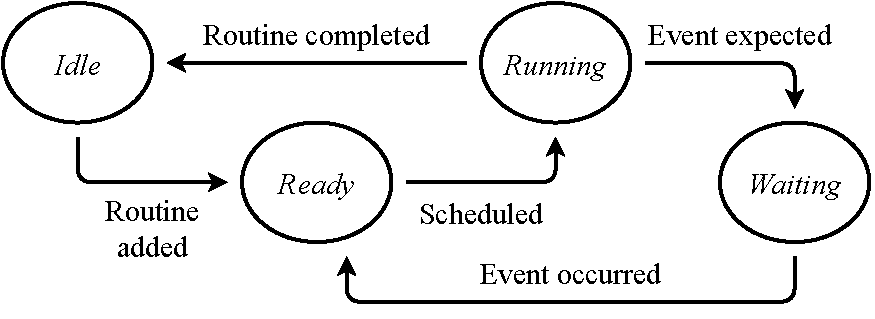
\includegraphics[width=0.6\textwidth]{figures/qnodeos/supplementary/process-states.pdf}
\end{center}
\caption[]{Process state diagram. An \emph{idle} process becomes \emph{ready} when a block for that process is loaded onto the \ac{QNPU} (from the \ac{CNPU}). A ready process becomes \emph{running} when it is scheduled. A running process goes back to idle if all blocks are completed, or transitions to \emph{waiting} if it expects an event to occur before it can proceed. A waiting process becomes ready again when the expected event occurs.}
\label{qnodeos:fig:process-states}
\end{figure}

\paragraph{QNPU process states}

A \ac{QNPU} process can be in any of the following states:
%
\begin{inlinelist}
\item \emph{Idle}: when the \ac{CNPU} has registered a program and the \ac{QNPU} has spawned a process, but it has not received a block yet;
\item \emph{Ready}: when it has (at least) one block, sent from the \ac{CNPU}, and can be scheduled and run;
\item \emph{Running}: when it is running on the \ac{QNPU} and has the quantum processor and the quantum network device assigned to it;
\item \emph{Waiting}: when it is waiting for some event to occur.
\end{inlinelist}
%
\Cref{qnodeos:fig:process-states} shows the possible process states and the valid state transitions. A process transitions from idle to ready when one block gets added. A ready process transitions to running when the the \ac{QNPU} scheduler assigns it to the processor. A running process transitions to waiting when it has to wait for an event to occur, and transitions from waiting to ready when the event occurs---for instance, a process could be waiting for an \ac{EPR} pair to be generated, and become ready again when the pair is established. Finally, a process goes back to the idle state when all its blocks have been completed.

\paragraph{Inter-process communication}

At the moment, the \ac{QNPU} does not allow for any explicit inter-process communication. The only indirect primitive available to processes to interact with one another is \emph{qubit ownership transfer}, used when a process produces a qubit state which is to be consumed by another process. Most notably, the quantum network stack kernel process transfers ownership of the entangled qubits that it produces to the process which requested the \ac{EPR} pairs.

\paragraph{Process concurrency}

The strict separation between local quantum processing and quantum networking is a key design decision in \ac{QNodeOS}, as it helps us address the scheduling challenge, see~\cref{qnodeos:sec:design-consid:challenges}. A user process can continue executing local instructions even after it has requested entanglement. Conversely, networking instructions can execute asynchronously of local quantum instructions. This is important in a quantum network, since entanglement generation must be synchronized with the neighboring node (and possibly the rest of the network~\cite{skrzypczyk_2021_arch}). Additionally, separating user programs into user processes also allows \ac{QNodeOS} to schedule several programs \emph{concurrently}.

\begin{figure}
\centering
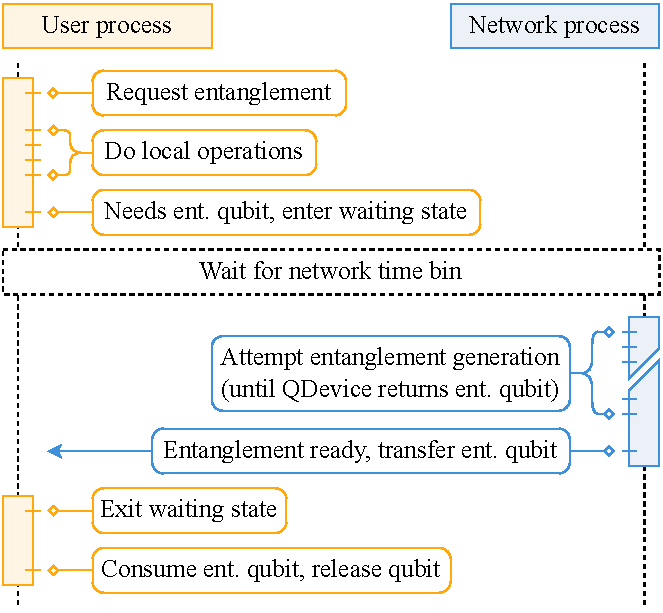
\includegraphics[width=0.6\textwidth]{figures/qnodeos/supplementary/process-flow.pdf}
\caption{Flow of execution between a user process requesting entanglement and the network process responsible for generating entanglement. The user process starts by asynchronously issuing an entanglement request. Once issued, it is free to continue with other local operations or classical processing. Once it reaches a point in its execution where entanglement is required the process enters the waiting state. The network process is scheduled once the appropriate time bin (as determined by the network schedule) starts. Once running, it attempts entanglement generation until entanglement success (or until a set timeout). The entangled qubit is then transferred to the user process. This unblocks the process which consumes the entanglement and releases the qubit. In our experiments, the process always immediately waits after requesting entanglement (no local operations are done in between).}
\label{qnodeos:fig:process-flow}
\end{figure}

\paragraph{Process flow}

\cref{qnodeos:fig:process-flow} illustrates the typical control flow between a user process and the network process. User processes are free to execute any non-networked instructions independently of the network process and other user processes. Once the program reaches a point in its execution where an entangled qubit is required, the process enters the waiting state and is flagged as waiting for entanglement. When the network process is scheduled, it issues network instructions and generates entanglement as requested by the user process. Once an entangled pair is generated by the network process, the qubit is handed over to the waiting user process. When all the entangled pairs that the user process was waiting for are delivered, the user process becomes ready and can start running again.

\subsubsection{Process Scheduling}
\label{qnodeos:sec:design:scheduling}

At present, the the \ac{QNPU} scheduler does not give any guarantees on when a process is scheduled---for that, one would need to define concrete real-time constraints to feed to the scheduler. Instead, the current version of the \ac{QNPU} implements a best-effort scheduler, which selects processes on the basis of their \emph{priority}, and does not allow preemption. In particular, the network process is assigned the highest priority, and is activated whenever the network schedule specifies entanglement should be made in the next time-bin~\cite{skrzypczyk_2021_arch}. 

As already mentioned, \ac{QNodeOS} defines the concept of \emph{user} processes and \emph{kernel} processes, with the \ac{QNetStack} process being the only kernel process at the moment. User processes are released (i.e., they become ready) asynchronously---when a process block is loaded, or when they leave the waiting state---while the \ac{QNetStack} process is released periodically---at the beginning of each time bin of the network schedule (although the period of time bins can vary). Given that generating an \ac{EPR} pair on a link requires that both nodes attempt entanglement simultaneously, the \ac{QNPU} assigns the \ac{QNetStack} process a priority higher than any user process. This ensures that, at the beginning of each time bin of the network schedule, the \emph{priority-based} process scheduler can assign the \ac{QNetStack} process as soon as the processor is available, and thus a node can start attempting entanglement with its neighbor as soon as possible and minimize wasted attempts on the neighbor node.

\Cref{qnodeos:fig:scheduling-impl} exemplifies a snapshot of a hypothetical execution of a user process and the \ac{QNetStack} process. The latter is activated at the beginning of a time-bin assigned to networking, and is scheduled as soon as the processor is available---for instance, at times $0$ and $4$ it is scheduled immediately, while at time $8$ it is scheduled after one time unit, as soon as the running process yields. The user process becomes ready at time $0$---at which point the \ac{QNetStack} process is ready as well and has highest priority, meaning the network process is scheduled; then it is scheduled at time $2$, as soon as the \ac{QNetStack} process completes; then it goes into waiting state at time $3$ because the user process requested entanglement and it waits for the entanglement to be established; finally it becomes ready again at time $7$---and it is scheduled immediately given that no other processes are running.

\begin{figure}
\begin{center}
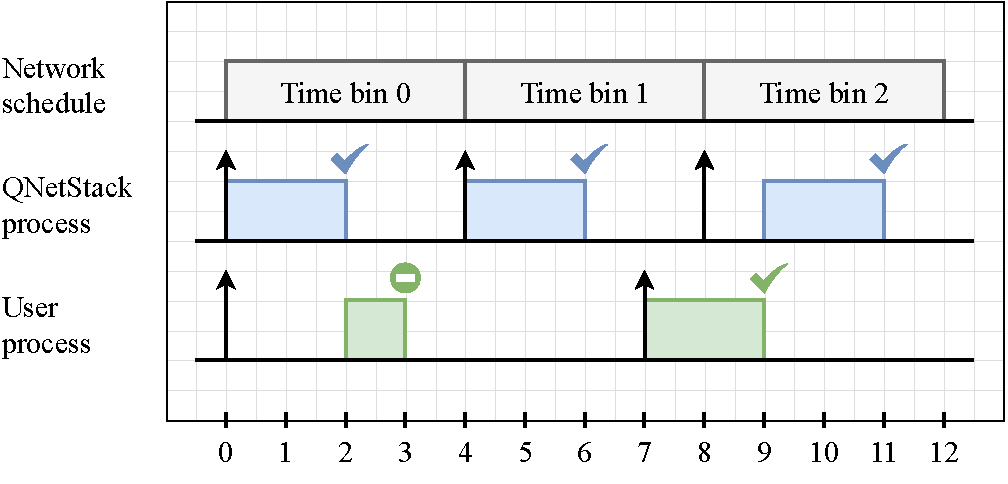
\includegraphics[width=0.7\textwidth]{figures/qnodeos/supplementary/scheduling-impl.pdf}
\end{center}
\caption[]{Snapshot of a hypothetical execution of a user process and the \ac{QNetStack} process. The higher-priority \ac{QNetStack} process is activated at the start of each time bin of the network schedule, and it is assigned to the processor as soon as it is available. The lower-priority user process gives precedence to the \ac{QNetStack} process when they become ready at the same time, but, when it is running on the processor, it is not preempted if the \ac{QNetStack} process becomes ready while the user process is running. Black arrows represents a moment where the process goes into the ready state and the green stop sign (at time $3$) represents a process going into the waiting state.}
\label{qnodeos:fig:scheduling-impl}
\end{figure}

To avoid context switching overhead, potentially leading to degraded fidelity, the \ac{QNPU} scheduler is \emph{cooperative}. That is, once a process is scheduled, it gets to run until it either completes all of its instructions or it blocks waiting for entanglement. Allowing process preemption would need a definition of critical section and could potentially impact the quality of the affected qubit states. Moreover, the lack of a preemption mechanism could potentially result in low-priority user processes hogging the processor at the expense of high-priority entanglement generation attempts. On the other hand, if entanglement instructions always consume the entirety of the time bin, the \ac{QNetStack} process would be immediately assigned the processor each time it relinquishes it, causing low-priority user processes to starve. To at least mitigate the second issue, we made sure that the number of consecutive entanglement attempts performed by the \ac{QDevice} within one single entanglement instruction is always less than how many would fit in a time bin, so as to leave some slack for low-priority user processes to run.

\subsubsection{Networking}
\label{qnodeos:sec:arch-networking}

The network stack \ac{QNetStack} is based on the existing stack~\cite{dahlberg_2019_egp}, including the link layer \ac{QEGP}~\cite{dahlberg_2019_egp}.
However the main difference between the \ac{QNetStack} implemented on the \ac{QNPU} and the original design of the protocols lies in how the \ac{QEGP} processes the outstanding entanglement requests. \ac{QEGP}~\cite{dahlberg_2019_egp} employed the concept of a distributed queue to sort and schedule entanglement requests on one node by coordinating with the counterpart node on the other end of the link, to ensure that both nodes would be servicing the same entanglement request at any given time. This synchronization is necessary because different entanglement requests may require different \ac{EPR} pair fidelities, in which case \ac{QEGP} would issue different \ac{QDevice} entanglement instructions. However, link-local request scheduling becomes more complicated if nodes have more than just one link. In that case, entanglement requests would be better scheduled at a level where network-wide request schedules are known. 

\paragraph{Network Schedule}
The \ac{QEGP} protocol implemented on the \ac{QNPU} transitioned~\cite{pompili_2022_experimental} from scheduling entanglement requests via a pairwise agreed upon distributed queue, to deferring this task to a \emph{logically centralized control plane}, whereby a node's schedule can be computed on the basis of the whole network's needs by a (logically) centralized controller (see e.g.~\cite{skrzypczyk_2021_arch}). This means that the network stack of the nodes convey their demands for end-to-end entanglement generation to the central controller, who then makes a \emph{network schedule}, which is communicated back to the nodes. 

All nodes divide time into time-bins, where the central controller employs a scheduling algorithm to assign either network actions (or no actions) to time-bins. That is, the term network schedule refers to a schedule, i.e. allocation of resources over time, of time-bins at the nodes, where a time-bin may be marked for networking activities (entanglement generation) or be left empty (to be used arbitrarily to execute local operations). 
Given that entanglement generation requires a non-deterministic amount of attempts and time, time bins are computed to be large enough to accommodate the average run time of an entanglement generation instruction. 
We remark that the node functions internally as a higher timing granularity than a time-bin allocated by the network scheduler, that is, it can execute other operations (such as for example local quantum operations) also within a time-bin allocated by the network schedule, provided entanglement is made early.

Once the node received the network schedule from the controller, the network schedule is used to satisfy all outstanding end-to-end entanglement requests, and is used by \ac{QEGP} to produce the correct \ac{QDevice} instructions at any point in time. Whenever a time bin is assigned to networking to two neighboring nodes, the nodes attempt entanglement generation over their shared link in order to realize the \ac{QEGP} link layer protocol. 
\Cref{qnodeos:fig:qnetstack-impl} shows internal components and data structures of the \ac{QNetStack} as it is implemented on the \ac{QNPU}. Entanglement requests received by the \ac{EMU} are forwarded by \ac{QNP} to the next hop's \ac{QNPU} system. Entanglement requests and network schedule---the latter installed by a logically centralized control plane---are used by \ac{QEGP} to produce the correct entanglement instructions to populate the \ac{QNetStack} process's block at each activation of the process.

\begin{figure}
\begin{center}
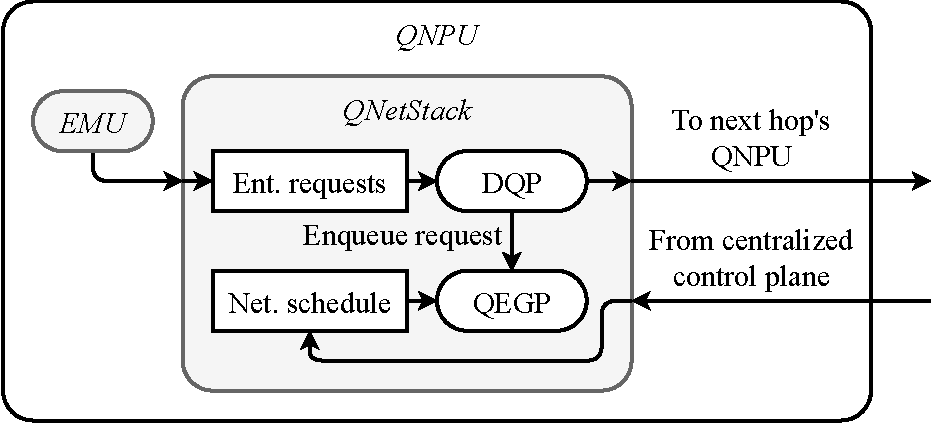
\includegraphics[width=0.6\textwidth]{figures/qnodeos/supplementary/qnetstack-impl.pdf}
\end{center}
\caption[]{Internal components and data structures of the \acf{QNetStack}. Entanglement requests are received through the \acf{EMU}, while the network schedule is installed by a centralized control plane. 
\acf{QEGP} maps such requests onto the network schedule to produce the correct entanglement instructions. While not needed on our 2 node implementation, a \ac{DQP} (which is a simplified version of the \ac{DQP} presented in~\cite[Section 5.2.1]{dahlberg_2019_egp}) could forward entanglement requests to the next hop's \acf{QNPU} to realize a network layer protocol such as~\cite{kozlowski_2020_qnp}.}.
\label{qnodeos:fig:qnetstack-impl}
\end{figure}

\paragraph{ER Socket}
\label{qnodeos:sec:design_er_socket}
The concept of an \ac{ER} socket is inspired by that of a classical network socket, in that it defines the endpoint of an entanglement generation request, and is used by the \ac{QNPU}'s quantum network stack to set up network tables and to establish connections with its peers. 
We remark that the current realization of the \ac{ER} Socket (see below) is a proof of concept implementation opening future computer science research, and does not aim to prevent misuse if different users had access to the same node. 
A program can request from QNodeOS the opening of an \ac{ER} socket with a program on a remote node. An \ac{ER} socket is identified by the tuple \texttt{(node\_id, er\_socket\_id, remote\_node\_id, remote\_er\_socket\_id)}. The other program (on the other node) must open its own corresponding \ac{ER} socket (i.e with values \texttt{(remote\_node\_id, remote\_er\_socket\_id, node\_id, er\_socket\_id)}) on its own QNodeOS. A request for opening an \ac{ER} socket is executed by the CNPU, by asking the QNPU (through the QNPU API) to open the socket. The QNPU then registers the ER socket with the quantum network stack (provided it did not yet exist), and the CNPU also keeps a reference using the tuple as an identifier. The program can then use this socket for requests. The network stack only handles requests for entanglement between two nodes if the corresponding \ac{ER} sockets are opened on both nodes.

Programs are themselves responsible for coordinating the ER socket IDs. Using these IDs allow the same node pair to open multiple pairs of ER sockets, which may be used by different applications or inside the same application. Socket IDs must be unique within the node. \ac{ER} sockets are typically opened at the start of a program, and live (and may be used multiple times) until the program finishes.

Programs use the \ac{ER} socket to submit entanglement requests to the network stack. This is done through NetQASM instructions (\texttt{create\_epr} and \texttt{recv\_epr}) that refer to the \ac{ER} socket in their operands. One program must execute a \texttt{create\_epr} instruction and the other a \texttt{recv\_epr} instruction (to be coordinated by the programs themselves). The program executing the \texttt{create\_epr} instruction is treated by the network stack as the \emph{initiator} and the program executing \texttt{recv\_epr} the \emph{receiver}. 
Upon receiving an entanglement request, the network stacks of the two nodes communicate between each other in order to coordinate entanglement generation. The initiator node always initiates this communication. The receiver node always accepts the entanglement initiative as long as the corresponding \ac{ER} socket is open. This means that the receiver node agrees with entanglement generation as soon as the initiator node has submitted an entanglement request (through its \texttt{create\_epr}), even if the receiver node itself has not yet submitted its corresponding request (through its \texttt{recv\_epr}). On the receiver node, the generated entangled qubit will remain in memory until it gets asked for by a user process executing this \texttt{recv\_epr}.

\subsubsection{Multitasking}

Multi-tasking forms an essential element of our architecture already at the level of scheduling the network process in relation to any user process, to address the challenges inherent in the way entanglement is produced at the physical layer, requiring agreement on a network schedule (see \cref{qnodeos:sec:arch-networking}). For this important reason, the \ac{QNPU} is designed to arbitrate between these two processes (see \cref{qnodeos:fig:process-flow}), and to manage the resources being used by each of them. \emph{Multitasking}, hence, is a fundamental requirement for a system managing the hardware of a quantum network node, especially while such hardware has only limited resources available. 

To further increase the utility of the system, we also allow the multi-tasking of user processes.
Like in most operating systems, these tasks, which on the \ac{QNPU} are encapsulated into processes, can sometimes necessitate a resource which is not immediately available---for instance, a free qubit, or a qubit entangled with a remote one. Maximizing the utilization of the quantum device is also one of the goals of \ac{QNodeOS}, whose design allows multiple processes, user and kernel, to be active concurrently, so that whenever one is in a waiting state, another one can potentially be scheduled to use the quantum device.  This design aspect is relevant for quantum networking nodes, as the execution of the local program is often waiting, both for classical messages from remote nodes, as well as the generation of entanglement. 

Lastly, multitasking is an important feature for systems that are to be shared by multiple users, and that offer each user the possibility to run multiple programs concurrently. The multitasking capabilities of \ac{QNodeOS} are also aimed at improving the average throughput and latency of user programs.


\subsection{QNodeOS Components and Interfaces}
\label{qnodeos:sec:appendix-qnodeos-core}

\begin{figure*}
\begin{center}
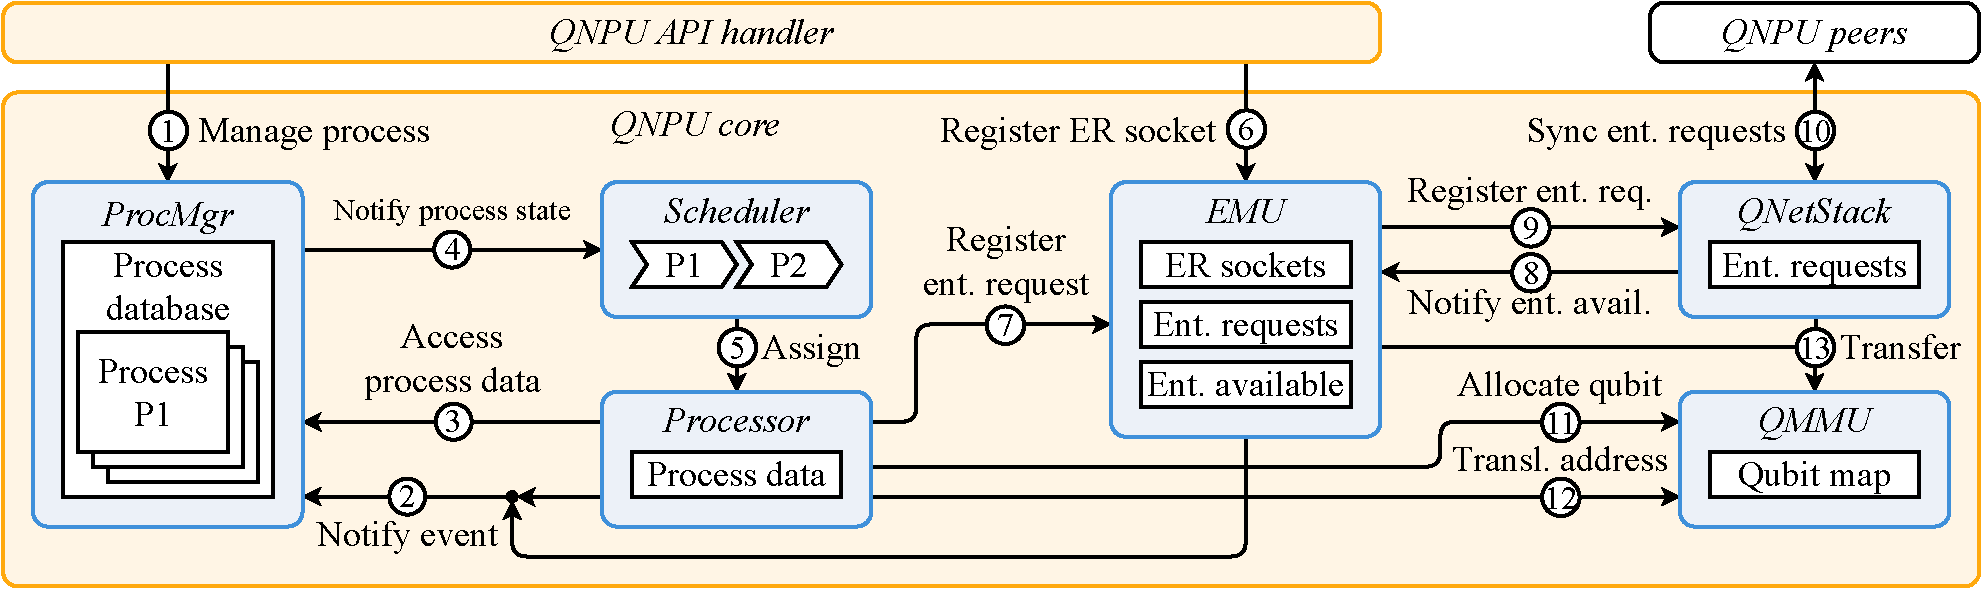
\includegraphics[width=1.0\textwidth]{figures/qnodeos/supplementary/qnodeos-core.pdf}
\end{center}
\caption[]{\acf{QNPU} core components and internal interfaces. The core layer includes:
\begin{inlinelist}
\item a \emph{process manager} (ProcMgr), which owns and manages access to \ac{QNPU} processes;
\item a \emph{scheduler}, responsible for selecting the next process to be run;
\item a \emph{processor}, which processes blocks' instructions;
\item an \emph{\ac{EMU}}, which keeps a list of entanglement requests and available entangled qubits;
\item a \emph{\ac{QNetStack}}, whose responsibility is to coordinate with peer nodes to schedule quantum networking instructions;
\item a \emph{\ac{QMMU}}, which keeps a record of allocated qubits.
\end{inlinelist}
}
\label{qnodeos:fig:qnodeos-core}
\end{figure*}

We provide here additional details on the components of the \ac{QNPU} architecture and their interfaces. \Cref{qnodeos:fig:qnodeos-core} gives an overview of all the components of the \ac{QNPU}. The \emph{process manager} marshals accesses to all user and kernel processes. The \emph{scheduler} assigns ready processes to the \emph{processor}, which runs quantum instructions through the underlying \ac{QDevice}, processes classical \ac{NetQASM} instructions locally, and registers entanglement requests with the \emph{\ac{EMU}}. The \ac{EMU} maintains a list of \ac{ER} sockets and entanglement requests, forwards the latter to the \emph{quantum network stack}, which, in turn, registers available entangled qubits with the \ac{EMU}. Finally, the \emph{\ac{QMMU}} keeps track of used qubits, and transfers qubit ownership across processes when requested.

\subsubsection{Process Manager}

The process manager owns \ac{QNPU} processes and marshals accesses to those. Creating a process, adding a block to it and accessing the process's data must be done through the process manager. Additionally, the process manager is used by other components to notify \emph{events} that occur inside the \ac{QNPU}, upon which the state of one of more processes is updated. Process state updates result in a notification to the scheduler.

\paragraph{Interfaces}

The process manager exposes interfaces for three services:
%
\begin{itemize}
\item Process management (interface 1 in \cref{qnodeos:fig:qnodeos-core}): to create and remove processes, and to add quantum blocks to them. When the user registers a program, the the \ac{QNPU} \ac{API} Handler uses the process manager to create a \ac{QNPU} user process. The returned process ID can be later used to add a block to that process, or to remove the process once all its blocks are fully processed.
\item Event notification (interface 2 in \cref{qnodeos:fig:qnodeos-core}): to notify an event occurred inside the \ac{QNPU}, including the addition of a block, the completion of a block, the scheduling of the process, the hitting of a \emph{Waiting} condition (see \cref{qnodeos:fig:process-states}), and the generation of an entangled qubit destined to the process. Some events trigger follow-up actions---for instance, when a process that was waiting for an event becomes ready, it gets added to the queue of ready processes maintained by the scheduler.
\item Process data access (interface 3 in \cref{qnodeos:fig:qnodeos-core}): to access a process's blocks and its classical memory space, mostly used while running the process (through the processor).
\end{itemize}

\subsubsection{Scheduler}

The \ac{QNPU} scheduler registers processes that are ready to be scheduled, and assigns them to the \ac{QNPU} processor when the latter is available. Ready processes are stored in a \emph{prioritized ready queue}, and processes of the same priority are scheduled with a first-come-first-served policy.

\paragraph{Interfaces}

The scheduler only exposes one interface for process state notifications (interface 4 in \cref{qnodeos:fig:qnodeos-core}), used by the process manager to signal when a process transitions to a new state. When a \ac{QNPU} process transitions to the ready state, it is directly added to the scheduler's prioritized ready queue. When a process becomes idle, or is waiting for an event to happen, the scheduler simply registers that the processor has become available.

\subsubsection{Processor}

The \ac{QNPU} processor handles the execution of \ac{QNPU} user and kernel processes, by running classical instructions locally and issuing quantum instructions to the \ac{QDriver}. It is also responsible for multitasking by means of process manager. While executing a process, the processor reads its blocks and accesses (reads and writes) its classical memory. The processor implements a specific instruction set architecture dictated by the \ac{NetQASM} language of choice.

\paragraph{Interfaces}

The processor exposes one interface for processor assignment (interface 5 in \cref{qnodeos:fig:qnodeos-core}), used by the \ac{QNPU} scheduler to activate the processor, when it is idling, and assign it to a \ac{QNPU} process.

\subsubsection{Entanglement Management Unit}

The \acf{EMU} contains a list of open \emph{\ac{ER} sockets} and a list of \emph{entanglement requests}, and keeps track of the \emph{available entangled qubits} produced by the quantum network stack. Received entanglement requests are considered valid only if an \ac{ER} socket associated to such requests exists. Valid requests are forwarded to the quantum network stack. Entangled qubit generations are notified as events to the process manager.

\paragraph{Interfaces}

The \ac{EMU} exposes interfaces for three services:
%
\begin{itemize}
\item \ac{ER} socket registration (interface 6 in \cref{qnodeos:fig:qnodeos-core}): to register and open \ac{ER} sockets belonging to a program, and to set up internal classical network tables and to establish classical network connection.
\item \ac{ER} registration (interface 7 in \cref{qnodeos:fig:qnodeos-core}): to add entanglement requests to the list of existing ones, to be used when matching produced entangled qubits with a process that requested them.
\item Entanglement notification (interface 8 in \cref{qnodeos:fig:qnodeos-core}): to register the availability of an entangled qubit, produced by the quantum network stack, and to link it to an existing entanglement request.
\end{itemize}

\subsubsection{Quantum Network Stack}

The quantum network stack on the \ac{QNPU} closely follows the model presented by
\textcite{dahlberg_2019_egp} which is based on the classical \ac{OSI} network stack model for the purpose of the separation of responsibilities. In particular, \emph{data link layer} is part of the quantum network stack on the \ac{QNPU}. The \emph{physical layer} is implemented on the \ac{QDevice}, the \emph{application layer} is part of the \ac{CNPU}, and all remaining layers are not currently part of the stack.

The quantum network stack component has an associated \emph{\ac{QNPU} kernel process}, created statically on the \ac{QNPU}. However, this process's block is dynamic: the instructions to be executed on the processor depend on the outstanding entanglement generation requests received from \ac{EMU} and network peers.

\paragraph{Interfaces}

The quantum network stack exposes interfaces for two services:
%
\begin{itemize}
\item Entanglement request registration (interface 9 in \cref{qnodeos:fig:qnodeos-core}): to add entanglement requests coming from the \ac{EMU} to the list of existing ones, which are used to fill in the quantum network stack process's block with the correct quantum instructions to execute.
\item Entanglement request synchronization (interface 10 in \cref{qnodeos:fig:qnodeos-core}): similar to the entanglement request registration interface, but to be used to synchronize (send and receive) requests with \ac{QNodeOS} network peers.
\end{itemize}

\subsubsection{Quantum Memory Management Unit}

\acf{QMMU} receives requests for \emph{qubit allocations} from \ac{QNPU} processes, and manages the subsequent usage of those. It also translates \ac{NetQASM} \emph{virtual qubit addresses} into physical addresses for the \ac{QDevice}, and keeps track of which process is using which qubit at a given time. In general, a \ac{QMMU} should take into account that the topology of a quantum memory determines what operations can be performed on which qubits, and thus allow processes to allocate qubits of a specific type upon request. An advanced \ac{QMMU} could also feature algorithms to move qubits in the background---that is, without an explicit instruction from a process's block---to accommodate a program's topology requirements while not trashing the qubits being used by other \ac{QNPU} processes. Such a feature could prove crucial to increase the number of processes that can be using the quantum memory at the same time, and to enhance multitasking performances.

\paragraph{Interfaces}

The \ac{QMMU} exposes interfaces for three services:
%
\begin{itemize}
\item Qubit allocation and de-allocation (interface 11 in \cref{qnodeos:fig:qnodeos-core}): a running process can ask for one or more qubits, which, if available, are allocated by the \ac{QMMU}, and the physical addresses of those are mapped to the virtual addresses provided by the requesting process.
\item Virtual address translation (interface 12 in \cref{qnodeos:fig:qnodeos-core}): before sending quantum instructions to the \ac{QDriver}, the processor uses virtual qubit addresses specified in \ac{NetQASM} to retrieve physical addresses from the \ac{QMMU}, and then replaces virtual addresses with physical addresses in the instructions for the \ac{QDriver}.
\item Qubit ownership transfer (interface 13 in \cref{qnodeos:fig:qnodeos-core}): qubits are only visible to the process that allocates them. However, in some cases, a process may wish to transfer some if its qubits to another one. A notable example is the quantum network process transferring an entangled qubit to the process that will use it.
\end{itemize}

\subsection{QNPU implementation: scheduler}
\label{qnodeos:sec:qnpu_impl_scheduler}
The \ac{QNPU} scheduler is an important component of our \ac{QNodeOS} architecture, and deals with scheduling of QNPU processes. The QNPU is implemented on FreeRTOS~\cite{freertos}, which itself includes a scheduler. On FreeRTOS, code is organized into tasks, which can be seen as separate threads or processes. These tasks are scheduled concurrently by FreeRTOS based on priority. In our implementation, we realize QNPU components and interfaces (hence including the QNPU scheduler) as FreeRTOS tasks. We configured task priorities such that the components with tight interaction with the QDevice (\ac{QDriver}, quantum network stack, QNPU processor) have highest priority.
We stress the difference between the FreeRTOS scheduler and our QNPU process scheduler. 
The QNPU scheduler schedules QNPU processes based on their status and priorities, which are independent of the priorities assigned by the FreeRTOS scheduler.
The FreeRTOS hence runs on a different layer: it makes sure the QNPU components (including QNPU scheduler, processor, \ac{QDriver}) run concurrently. The QNPU scheduler runs on the level of QNPU processes. Whenever the FreeRTOS scheduler activates the FreeRTOS task realizing the QNPU scheduler, the QNPU scheduler then schedules the process with the highest priority on a first come first serve basis, by adding it to the processing queue of the relevant resource (e.g. QNPU processor) and generating an interrupt leading to the execution of the QNPU processor task on FreeRTOS (and consequently the execution of the process).

\subsection{QDevice Interface}
\label{qnodeos:sec:appendix-qdevice}

The implementation of a \ac{QDevice} depends on a number of factors. Most importantly, the physical signals that are fed to the quantum processing and networking device (and those that are output from the device) are specific to the nature of the device itself. Different qubit realizations require different digital and analog control. For instance, manipulating the state of a spin-based qubit (e.g., in a \ac{NV} center processor) and that of an atom qubit (e.g., in a trapped ion processor) are two physical processes that vastly differ in a number of complex ways.

For \ac{QNodeOS} to be portable to a diverse set of quantum physical platforms, there needs to be a common \emph{\ac{QDevice} interface} that \ac{QNodeOS} can rely on, and that each \ac{QDevice} instance can implement as it is most convenient for the underlying quantum device. This interface \begin{inlinelist} \item needs to be \emph{general}, \item to be able to \emph{express all quantum operations} that different quantum devices might be capable of performing, and \item \emph{abstract}, so that two different implementations of a well-defined qubit manipulation operation can be expressed with the same instruction on \ac{QNodeOS}.\end{inlinelist} Nevertheless, an interface that is too general could result in a high implementation complexity on the \ac{QDevice}, as it might have to transform high-level instructions in a series of native operations on the fly. Other than complexity of implementation, a very high-level set of \ac{QDevice} instructions might compromise the compiler's ability to optimize a program for a certain physical platform, as reported by~\textcite{murali_2019_fullstack}.

\subsubsection{Design Choices}

Defining a set of instructions to express abstract quantum operations as close as possible to what different quantum physical platforms can natively perform is---to some extent---an open problem. Nonetheless, we have made an effort to specify an interface which is a good compromise between generality and expressiveness. The \ac{QDevice} interface is essentially a set of instructions that \ac{QNodeOS} expects a \ac{QDevice} to implement. To be precise, a \ac{QDevice} might implement a subset of the interface, according to what native physical operations it can perform. The CNPU compiler must then have knowledge about the set of instructions implemented by the underlying \ac{QDevice}, so that it can decompose instructions that are not natively supported.

Even though this interface does not impose any formal timing constraints, it is important to note that a \ac{QDevice} implementation that tries to guarantee more or less deterministic instruction processing latencies can prove more beneficial to the real-time requirements of the \ac{QNPU}. Particularly, it would be advisable to time-bound the processing time of operations whose duration is by nature probabilistic---most notably, those involving entanglement generation. Creating an \ac{EPR} pair may involve a varying number of attempts. Sometimes, if the remote node becomes unresponsive for some time, the number of necessary attempts can increase by a large amount. Capping the number of attempts could, for instance, provide a more deterministic maximum processing latency for entanglement instructions, which in turn might help \ac{QNodeOS} react more timely to temporary failures or downtime periods of remote nodes. Not to mention that unbounded entanglement attempts affect the state of other qubits in memory, because of both passive decoherence and cross-qubit noise.

\subsubsection{QDevice synchronization}
\label{qnodeos:sec:qdevice-sync}
The QDevice receives physical instructions from QNodeOS, acts on them, and returns a response. For entanglement instructions, the QDevice must first synchronize with the QDevice on the other node (using classical communication). If the other QDevice is busy, (e.g. it is still trying to pass the CR check, see~\cref{qnodeos:sec:qdevice-nv} and \cite{pompili_2022_experimental}), synchronization fails, and an \texttt{ENT\_SYNC\_FAIL} response is returned (see~\cref{tab:qdevice-return-values}).

\subsubsection{Instructions and Operands}
\label{qnodeos:sec:appendix-qdevice-instructions-operands}

\begin{table}[t]
\begin{tabularx}{\linewidth}{>{\ttfamily}l X}
\toprule
\normalfont{Instruction} & Description \\
\midrule
INI & Initialize a qubit to default state \\
SQG & Perform a single-qubit gate \\
TQG & Perform a two-qubit gate \\
AQG & Perform a gate on all qubits \\
MSR & Measure a qubit in a specified basis \\
ENT & Attempt entanglement generation \\
ENM & Attempt entanglement and measure qubit \\
MOV & Move qubit state to another qubit \\
SWP & Swap the state of two qubits \\
ESW & Swap qubits belonging to two \ac{EPR} pairs \\
PMG & Set pre-measurement gates \\
\bottomrule
\end{tabularx}
\caption[]{Summary of \ac{QDevice} instructions defined in the \ac{QDevice} interface. A specific \ac{QDevice} might implement a subset of these, depending on the underlying quantum physical device and on other design constraints.}
\label{tab:qdevice-instructions}
\end{table}

\Cref{tab:qdevice-instructions} lists the complete set of instructions defined in the \ac{QDevice} interface. Instructions can have operands, whose range of valid values depends on the underlying \ac{QDevice}. For instance, an operand that specifies which qubit to apply an operation to can only have as many valid values as there are physical qubits in memory. Details for each instruction and its operands are given below.

\paragraph{Qubit Initialization (\texttt{INI})}

The \texttt{INI} instruction brings a qubit to the $\ket{0}$ state. On some physical platforms, single-qubit initialization is not possible, thus this instruction initializes all qubits to the $\ket{0}$ state.

\medskip \noindent
\begin{tabularx}{\linewidth}{>{\ttfamily}l X}
\toprule
\normalfont{Operand} & Description \\
\midrule
qubit & Physical address of the qubit to initialize, ignored on platforms where single-qubit initialization is not possible \\
\bottomrule
\end{tabularx}

\paragraph{Single-Qubit Gate (\texttt{SQG})}

The \texttt{SQG} instruction manipulates the state of one qubit. The gate is expressed as a rotation in the Bloch sphere.

\medskip \noindent
\begin{tabularx}{\linewidth}{>{\ttfamily}l X}
\toprule
\normalfont{Operand} & Description \\
\midrule
qubit & Physical address of the qubit to manipulate \\
axis  & Rotation axis, can be X, Y, Z or H (support is \ac{QDevice}-dependent) \\
angle & Rotation angle (granularity and range are \ac{QDevice}-dependent) \\
\bottomrule
\end{tabularx}

\paragraph{Two-Qubit Gate (\texttt{TQG})}

The \texttt{TQG} instruction manipulates the state of two qubits. The gate is expressed as a controlled rotation, with one qubit being the control and the other one being the target.

\medskip \noindent
\begin{tabularx}{\linewidth}{>{\ttfamily}l X}
\toprule
\normalfont{Operand} & Description \\
\midrule
qub\_c & Physical address of the control qubit \\
qub\_t & Physical address of the target qubit \\
axis   & Rotation axis, can be X, Y, Z or H (support is \ac{QDevice}-dependent) \\
angle  & Rotation angle (granularity and range are \ac{QDevice}-dependent) \\
\bottomrule
\end{tabularx}

\paragraph{All-Qubit Gate (\texttt{AQG})}

The \texttt{AQG} instruction manipulates the state of all available qubits. The gate is expressed as a rotation in the Bloch sphere.

\medskip \noindent
\begin{tabularx}{\linewidth}{>{\ttfamily}l X}
\toprule
\normalfont{Operand} & Description \\
\midrule
axis  & Rotation axis, can be X, Y, Z or H (support is \ac{QDevice}-dependent) \\
angle & Rotation angle (granularity and range are \ac{QDevice}-dependent) \\
\bottomrule
\end{tabularx}

\paragraph{Qubit Measurement (\texttt{MSR})}

The \texttt{MSR} instruction measures the state of one qubit in a specified basis. A qubit measurement is destructive---that is---the qubit has to be reinitialized before it can be used again.

\medskip \noindent
\begin{tabularx}{\linewidth}{>{\ttfamily}l X}
\toprule
\normalfont{Operand} & Description \\
\midrule
qubit & Physical address of the qubit to measure \\
basis & Measurement basis, can be X, Y, Z, H (support is \ac{QDevice}-dependent) \\
\bottomrule
\end{tabularx}

\paragraph{Entanglement Generation (\texttt{ENT})}

The \texttt{ENT} instruction performs a series of entanglement generation attempts, until one succeeds, or until a maximum number of attempts is reached (the behavior is \ac{QDevice}-dependent).

\medskip \noindent
\begin{tabularx}{\linewidth}{>{\ttfamily}l X}
\toprule
\normalfont{Operand} & Description \\
\midrule
nghbr & Neighboring node to attempt entanglement with, if the local \ac{QDevice} has multiple quantum links \\
fid & Target entanglement fidelity (granularity and range are \ac{QDevice}-dependent) \\
\bottomrule
\end{tabularx}

\paragraph{Entanglement Generation With Qubit Measurement (\texttt{ENM})}

The \texttt{ENM} instruction performs a series of entanglement generation attempts followed by an immediate measurement of the local qubit, until one succeeds, or until a maximum number of attempts is reached (the behavior is \ac{QDevice}-dependent).

\medskip \noindent
\begin{tabularx}{\linewidth}{>{\ttfamily}l X}
\toprule
\normalfont{Operand} & Description \\
\midrule
nghbr & Neighboring node to attempt entanglement with, if the local \ac{QDevice} has multiple quantum links \\
fid & Target entanglement fidelity (granularity and range are \ac{QDevice}-dependent) \\ basis & Measurement basis, can be X, Y, Z, H (support is \ac{QDevice}-dependent) \\
\bottomrule
\end{tabularx}

\paragraph{Qubit Move (\texttt{MOV})}

The \texttt{MOV} instruction moves the state of one qubit to another qubit. A qubit move renders the state of the source qubit undefined, and the qubit has to be reinitialized before it can be used again.

\medskip \noindent
\begin{tabularx}{\linewidth}{>{\ttfamily}l X}
\toprule
\normalfont{Operand} & Description \\
\midrule
qub\_s & Physical address of the source qubit \\
qub\_d & Physical address of the destination qubit \\
\bottomrule
\end{tabularx}

\paragraph{Qubit Swap (\texttt{SWP})}

The \texttt{SWP} instruction swaps the state of two qubits.

\medskip \noindent
\begin{tabularx}{\linewidth}{>{\ttfamily}l X}
\toprule
\normalfont{Operand} & Description \\
\midrule
qub\_1 & Physical address of the first qubit \\
qub\_2 & Physical address of the second qubit \\
\bottomrule
\end{tabularx}

\paragraph{Entanglement Swap (\texttt{ESW})}

The \texttt{ESW} instruction results in two qubits belonging to two \ac{EPR} pairs to have their roles swapped.

\medskip \noindent
\begin{tabularx}{\linewidth}{>{\ttfamily}l X}
\toprule
\normalfont{Operand} & Description \\
\midrule
qub\_1 & Physical address of the first qubit \\
qub\_2 & Physical address of the second qubit \\
\bottomrule
\end{tabularx}

\paragraph{Pre-Measurement Gates Setting (\texttt{PMG})}

The \texttt{PMG} instruction allows for a set of (up to) 3 rotations to be performed before a qubit measurement (\texttt{MSR} or \texttt{ENM}). If the axis of the second rotation is orthogonal to the axis of the first and the third rotation, these gates can be used to perform a qubit measurement in an arbitrary basis, given that most likely a \ac{QDevice} can natively measure in a limited set of bases.

\medskip \noindent
\begin{tabularx}{\linewidth}{>{\ttfamily}l X}
\toprule
\normalfont{Operand} & Description \\
\midrule
axes & Combination of orthogonal axes to use for the three successive rotations, can be X--Y--X, Y--Z--Y and Z--X--Z (support is \ac{QDevice}-dependent) \\
ang\_1 & Rotation angle of the first gate, relative to the first axis in \texttt{axes} (granularity and range are \ac{QDevice}-dependent) \\
ang\_2 & Rotation angle of the second gate, relative to the second axis in \texttt{axes} (granularity and range are \ac{QDevice}-dependent) \\
ang\_3 & Rotation angle of the third gate, relative to the third axis in \texttt{axes} (granularity and range are \ac{QDevice}-dependent) \\
\bottomrule
\end{tabularx}

\paragraph{No operation (\texttt{NOP})}

The \texttt{NOP} instruction does not result in any operation on the \ac{QDevice}.

\subsubsection{Return values}
\Cref{tab:qdevice-return-values} lists the possible return values that the QDevice sends back to QNodeOS as a response to a physical instruction.

\begin{sidewaystable*}[t]
    \centering
    \begin{tabularx}{\textwidth}{|l|l|X|}
    \hline
    Physical Instruction & Return values & Description \\ 
    \hline
    \texttt{INI}, \texttt{SQG}, \texttt{TQG}, \texttt{AQG}, \texttt{PMG} & \texttt{SUCCESS} & Always successful \\
    \texttt{MSR} & \texttt{SUCCESS\_0} or \texttt{SUCCESS\_1} & Measurement outcome is 0 or 1* \\ 
    \texttt{ENT} & \texttt{SUCCESS\_<state>} & Entanglement generation was successful; the state is <state>$^\dagger$ \\
    \texttt{ENM} & \texttt{SUCCESS\_<state>\_<outcome>} & Entanglement generation was successful; state was <state>$^\dagger$ and outcome is <outcome> (0 or 1) \\
    \texttt{ENT, ENM} & \texttt{ENT\_FAILURE} & Entanglement generation was attempted and failed \\
    \texttt{ENT, ENM} & \texttt{ENT\_SYNC\_FAILURE} & Entanglement generation was not attempted since synchronization failed (other node is busy) \\
    \hline
    \end{tabularx}
    \caption{*Measurements are always in the Z basis, where outcome 0 corresponds to $\ket{0}$ and outcome 1 to $\ket{1}$. $^\dagger$ Possible states depend on the implementation. For NV these are \texttt{PSI\_PLUS} and \texttt{PSI\_MINUS}, see~\cref{qnodeos:sec:qdevice-nv}.}
    \label{tab:qdevice-return-values}
\end{sidewaystable*}
